\documentclass[11pt, english, fleqn, DIV=15, headinclude, BCOR=2cm]{scrreprt}

\usepackage[
    color,
    bibatend,
]{../../header}

\graphicspath{{./}{../Figures/}}

\usepackage{needspace}

\usepackage{mathtools}
\usepackage{listings}

\lstset{
    basicstyle=\small\ttfamily,
}

\hypersetup{
    pdftitle=
}

\newcommand\mot{\textsc{mot}}

\usepackage{longtable}
\usepackage{subcaption}

\usepackage[all]{nowidow}

\DeclareMathOperator\sinc{sinc}

\subject{Lab report}
\title{Optical frequency doubling}
\subtitle{Experiment A245 -- Universität Bonn}
\author{%
    Martin Ueding \\
    \small{\href{mailto:mu@martin-ueding.de}{mu@martin-ueding.de}}
    \and
    Lino Lemmer \\
    \small{\href{mailto:l2@uni-bonn.de}{l2@uni-bonn.de}}
}

\date{\daterange{2016-05-23}{2016-05-24}}

\publishers{Tutor: Gautam Ramola}

\begin{document}

\maketitle

\begin{abstract}
\end{abstract}

\tableofcontents

\chapter*{Permission to upload}

I, Martin Ueding, would like to scan and upload this lab report with your
corrections to my website \href{http://martin-ueding.de}{martin-ueding.de}.
There, the original lab report as well as the reviewed one will be licensed
under the “\href{http://creativecommons.org/licenses/by-sa/4.0/}{Creative
Commons Attribution-ShareAlike 4.0 International License}”. Is that okay with
you?

Yes $\Box$ \hspace{2cm} No $\Box$

\chapter{Theory}

\section{Generation of harmonics}

This section follows the work by
\textcite[Chapter~12]{meschede/optik_licht_laser/2008}.

A normal driven harmonic oscillator obeys the differential equation for the
force,
\[
    \ddot x + \omega_0^2 x = \frac qm \mathcal E \cos(\omega t) \,,
\]
where $x(t)$ is the position of the oscillating particle, $\omega_0^2$ the
eigenfrequency of the system, $q/m$ the specific electric charge, $\mathcal E$
the driving field amplitude and $\omega$ the external driving frequency. The
solutions of this equation are harmonics with frequency!$\omega$ and a certain
amplitude which depends on the distance of $\omega$ from $\omega_0$.

The linear force is a good approximation until ones uses high intensity laser
beams. Then one needs to include the next term in the force expansion, $\alpha
x^2$. For $\alpha \ll 1$ we can neglect $\alpha^2$ terms. The solution~$x(t)$
will then consist of two summands, the first is the already known harmonic with
$\omega$: $x^{(1)}(t) = x_\text l \cos(\omega t)$ with $x_\text l$ the
amplitude of the linear part. The second summand, suppressed by $\alpha$ will
approximately obey the differential equation
\[
    \ddot x^{(2)} + \omega_0^2 x^{(2)} \simeq - \alpha x_\mathrm l^2
    \cos(\omega t)^2 \,.
\]
Using the relation $\cos(\omega t)^2 = 1/2 + \cos(2 \omega t)/2$ we see that
there will be a constant part and a part oscillating with $2 \omega$. The
amplitude of that part has to be derived.

By looking at the propagation of waves in the non-linear medium one can derive
a differential equation for each polarization induced by the incoming and
outgoing waves. With the assumption of nearly plane waves one can simplify to a
one dimensional differential equation. Setting the incoming waves to the same
frequency they boil down to two equations.

In our case the conversion will only be week. The light passes the crystal only
once, we only have the length $l$ to generate the harmonic. Therefore the
fundamental wave can be assumed to be constant. The important result is the
intensity of the harmonic:
\[
    I_\text h = \underbrace{\frac{4 d_\text{eff}^2 \omega^2}{c^3 \varepsilon_0
    n_\omega^2 n_{2\omega}}}_{\Gamma^2} l^2 I_\mathrm f^2 \sinc(\Deltaup k l /
    2)^2 \,.
\]
We choose the non-normalized variant $\sinc(x) = \sin(x)/x$. $\Gamma$ contains
all the material quantities. Here one can see that $|\Delta k|$ must be small
such that a large harmonic intensity is generated.

\section{Birefringence}

Most materials are sufficiently isotropic; their refractive index does not
depend on the propagation direction. Birefringent materials have a refractive
index that does depend on the direction of propagation and the polarization.
This makes for interesting effects.

The simplest manifestation of the effect are uniaxial crystals. They have one
\emph{extraordinary} direction and two \emph{ordinary} directions. The
extraordinary direction is called the \emph{optical axis} of the crystal. If a
beam is polarized in parallel to the extraordinary axis, it will be governed by
the refractive index $n_\mathrm e$. Its propagation direction must be
orthogonal to the to the optical axis. If the polarization is along one of the
ordinary directions, it can propagate in any direction through the crystal. The
refractive index for this is called $n_\mathrm o$.

A beam which has polarization projections on both ordinary and extraordinary
directions will exhibit two different refractive indices. Different refractive
indices imply different phase velocities and can therefore alter the overall
polarization, shape and propagation direction of the beam.

In this experiment we will use a crystal which has a different refractive index
along each of the three spatial directions. As long as we use it along one of
the directions we only see two different indices anyway; light cannot be
polarized longitudinally.

One important application are \emph{retarder plates} which can conveniently
change the polarization. Both important kinds are cut such that the optical
axis is orthogonal to the propagation direction. By rotating it one can mix the
polarization components as needed.

The first kind is the $\lambda/2$-plate. Incoming linearly polarized light will
hit the plate with an angle $\phi$ between polarization and optical axis. The
polarization component parallel to the optical axis will be advanced or
retarded (depending whether $n_\mathrm o$ is larger or smaller than $n_\mathrm
e$) and ultimately rotate the polarization direction by the angle $2 \phi$
\parencite[Figure~3.20]{meschede/optik_licht_laser/2008}. This way one can
effectively rotate the linear polarization freely.

The second kind is the $\lambda/4$-plate. This one can be used in two ways.
Incoming linear polarized light hitting the plate with an angle $\phi =
\SI{45}{\degree}$ between polarization and optical axis will become circularly
polarized \parencite[Figure~3.20]{meschede/optik_licht_laser/2008}. The other
way around one can convert circular polarization into linear one. If one
chooses a different angle, the light will be just elliptically polarized.

\section{Phase matching}

This section follows the work by
\textcite[Section~12.4.3]{meschede/optik_licht_laser/2008}.

As one has seen in the section about the generation of harmonics, the phase
difference $\Deltaup k$ determines the strength of the second harmonic. The
best results are obtained for $\Deltaup k = 0$. With \emph{phase matching}, one
can tune $\Deltaup k \approx 0$. Since we have
\[
    \Deltaup k
    = k_{2\omega} - 2 k_\omega
    = \frac{2\omega}{c} (n_{2\omega} - n_\omega) \,,
\]
the phase difference depends on the difference in the refractive index~$n$ at
the given frequency
\parencite[Equation~(12.12)]{meschede/optik_licht_laser/2008}. The idea is to
give the fundamental and harmonic frequency the same refractive index such that
$\Deltaup k = 0$. By using birefringent materials one has a different
refractive index depending on the polarization and direction through the
crystal.

Crystals used for frequency conversion have a normal dispersion relation. This
means that the refractive index is lower for higher wavelength. In order to
match the refractive indices of $\omega$ (large wavelength) and $2\omega$
(small wavelength), one has to choose the larger refractive index for the
fundamental wave and the smaller one for the harmonic. Depending on the crystal
one might have $n_\mathrm o < n_\mathrm e$ (called \emph{positive}) or
$n_\mathrm o > n_\mathrm e$ (called \emph{negative}).

Using the phase difference one can define a \emph{coherence length}
$l_\text{coh} = \piup/\Deltaup k$ which gives the distance over which the
harmonic amplitude oscillates
\parencite[Equation~(12.14)]{meschede/optik_licht_laser/2008}. For typical
crystals without intervention one finds $l_\text{coh} \simeq
\SI{10}{\micro\meter}$
\parencite[Section~12.4.1]{meschede/optik_licht_laser/2008}. This means that we
definitely have to match the phases in order to get significant light output.


\subsection{Type 1 and 2}

We will only describe the case of negative uniaxial crystals here. For a
positive uniaxial crystal one just takes perpendicular polarizations. As we are
in a negative crystal we have $n_\mathrm o > n_\mathrm e$. As the fundamental
wave has to take the larger refractive index, which is the \emph{ordinary}
direction. The harmonic wave must be---at least partially---in the
extraordinary direction.

We have two choices to choose the incoming polarization. Choosing the
polarization of the fundamental wave to be purely ordinary we can only combine
two photons of the ordinary direction into one photon of the extraordinary
direction. This is called \emph{type 1 phase matching}. The other way is to
choose a \SI{45}{\degree} angle of the fundamental wave. It will have equal
parts which propagate in the ordinary and extraordinary direction. One photon
of each direction can then be combined into one harmonic photon. That way is
called \emph{type 2 phase matching}.

In a real crystal it would be an unlikely coincidence that the refractive
indices for ordinary and extraordinary transmission are exactly equal at
$\omega$ and $2\omega$. Therefore one needs one degree of freedom to adjust.

\subsection{Angle adjustment}

Every crystal can be tilted such that the angle between the optical axis of the
crystal and the incoming light is $\pi/2 + \theta$. A better way is to say that
the surface normal of the optical table forms an angle $\theta$ with the
optical axis of the crystal. By tilting the crystal one can can tune the
effect refractive index of the extraordinary direction. We then have
\[
    \frac1{n_\mathrm e(\theta)}
    = \frac{\cos(\theta^2)}{n_\mathrm o^2}
    + \frac{\sin(\theta^2)}{n_\mathrm e^2} \,,
\]
as given by \textcite[Equation~(3.31)]{meschede/optik_licht_laser/2008}. Given
the refractive indices one can then find the optimal angle for the crystal. One
problem with this method is the \emph{walk-off} as the harmonic light now has
the same phase velocity but not necessarily the same direction.

We do not use this method in our experiment as we have something fancier.

\subsection{90 degree adjustment}

The \emph{\SI{90}{\degree} adjustment} or \emph{temperature adjustment} does
not have the problem of walk-off. One uses $\theta = 0$ in order to have
perfectly perpendicular propagation directions. In order to fine-tune the
refractive indices one uses a temperature dependence. So instead of matching
via tilt one does via temperature dependence. The material used in our
experiment, $\mathrm{KNbO_3}$ has a sufficient temperature dependence to allow
phase matching for frequency doubling in the range
\SIrange{950}{1060}{\nano\meter} for a b-cut crystal. This \enquote b refers to
the cut direction. This crystal material has different refractive indices in
all three directions (\enquote a, \enquote b and \enquote c), therefore one can
choose the frequency range to work with.

\section{Gaussian beams}

This section follows the work by
\textcite[Section~12.4.4]{meschede/optik_licht_laser/2008}.

A Gaussian light beam is a good approximation to the beams that we can create
with a laser. It has a Gaussian electric field intensity distribution. When one
focuses the beam it will have a smallest point, the waist. There the beam
radius is $w_0$.
\[
    \mathcal E(r) = \mathcal E_0 \exp(-(r/w_0)^2) \,,
\]
The \emph{Rayleigh length}~$z_0$ is the distance from the focus point where the
beam cross sectional area has doubled. The \emph{confocal parameter} $b$ is
just twice the Rayleigh length: $b = 2 z_0$.

The diameter of a Gaussian beam given by \parencite{wikipedia/gaussian_beam} as
\[
    w(z) = w_0 \sqrt{1 + \frac{z^2}{z_0^2}} \,.
\]
Together with the relation
\[
    z_0 = \frac{n \piup \omega_0^2}{\lambda_0}
\]
from \parencite{wikipedia/rayleighleange} only one free parameter is left.

Introducing the focusing into the expected harmonic power, one obtains
\[
    P_\mathrm h
    = \frac{\Gamma^2 l^2 P_\mathrm f^2}{\piup w_\mathrm h^2} \frac1\xi h(0,
    \xi) \,.
\]
Here $l$ is the crystal length, $\xi = l / b$ is the \emph{normalized crystal
length} and $h(0, \xi)$ is the Boyd-Kleinman reduction factor in the case of
\SI{90}{\degree} phase matching. For $\xi_0 = 2.84$ the function $h(0, \xi)$
obtains its maximum value of \num{1.068}.

\section{Wavelength measurement}

In this experiment we want to double the frequency of light. In order to verify
that it works we need a way to measure the frequency. Although that is in
principle doable with the \emph{optical comb} we choose the easier route by
measuring the wavelength and convert with the speed of light.

\subsection{Gratings}

A practical way to measure the wavelength are \emph{gratings} which are
available for use in reflection and transmission. A CD or DVD is a readily
available example of a reflection grating. We will use a regular grating which
has parallel lines.

% TODO Drawing of a grating?

The basic idea is that the light is only transmitted or reflected through a
large number of thin slits. By the principle of Huygens each of the lines will
create a cylindrical wave which interferes with the other ones. At an angle
$\phi$ the different waves will interfere with a phase shift $\Deltaup k$ which
depends on the different lengths traveled. For some $\phi$ it will give
constructive interference. The $n$-th order of the wavelength~$\lambda$ is
scattered into an angle~$\phi_n$ governed by
\[
    \sin(\phi_n) = \frac{n \lambda}{g} \,,
\]
with line distance $g$ \parencite{wikipedia/optisches_gitter}. This equation
only holds for incoming light that is perpendicular to the grating.

The resolution of the grating is given by
\[
    \frac{\lambda}{\Deltaup \lambda} = n N \,,
\]
with the number of illuminated lines~$N$
\parencite{wikipedia/optisches_gitter}. The resolution of a grating is quite
good but there are even better ways.

\subsection{Michelson interferometer}

% The \emph{Michelson interferometer} is a very precise measuring apparatus 

% TODO Drawing of a Michelson interferometer?

With the positions $d_1$ and $d_2$ of the end mirrors one obtains a phase
difference between the arms of $\delta = 4 \piup [d_1 - d_2] / \lambda$
\parencite[559]{meschede-gerthsen_24}. The intensity of the beam reaching the
detector is given by \textcite[559]{meschede-gerthsen_24} as
\begin{equation}
    \label{eq:I_of_lambda}
    I(\lambda) = \frac12 I_0(\lambda) \sbr{
        1 +
        \cos\del{4 \piup \frac{d_1 - d_2}{\lambda}}
    } \,.
\end{equation}
For the exact same arm lengths one does not see any difference between
different wavelengths. We will use $d_1 \neq d_2$ and move one of the mirrors,
say the first. Then by changing $d_1$ we will change $I(\lambda)$. For a
constant $\dot d_1$ we will see a different $\dot I(\lambda)$ and $\dot
I(\lambda/2)$.

% TODO What is the resolution of this thing?

\section{Diode laser}
\label{sec:diode_laser}

A laser is a light generation element which works with an occupation inversion
in the laser states. Most atoms are in the excited state and will decay when a
resonant photon hits them. This way coherent light is created which will get
stronger the more atoms it passes. Various laser differ by the pumping
mechanism and the manifestation of the resonator.

The \emph{diode laser} is a junction of two differently (positively and
negatively) doped semiconductors. The zone in between will become depleted on
its own. By applying a voltage one can inject electrons and holes from either
side of the junction. In the middle those annihilate and emit photons if the
semiconductor has the proper transition possibilities. The semiconductor chip
serves as a resonator to amplify the stimulated emission.

Without any further adjustments, the laser spectrum will be quite broad. We
want a single mode laser for our experiment, therefore we need to \emph{lock}
the laser. In the \emph{Littrow configuration} one uses a reflection grating to
reflect the $-1$-th order back onto the laser diode. The laser diode and the
grating form an \emph{external resonator}. By adjusting the angle of the
grating one can effectively choose the resonant frequency of the resonator. The
light output is reflected away by the zeroth order of the grating. By driving
the grating with Piezo crystals one can tune the laser at will. Feeding the
output signal into a control circuit allows to lock the laser to a fixed
frequency which is robust against temperature changes or vibrations.

Due to the shape of the junction, the beam shape will have an elliptical shape.
One has to adjust this in order to get a circular beam shape.

\chapter{Conduction and analysis}

\section{Diode laser classification}

First we want to classify the Laser diode at hand. We have a diode laser which
is mounted behind a safety shutter. One of the characteristics of a diode laser
is the elliptical beam shape as described in Section~\ref{sec:diode_laser}
already. Therefore our setup includes a pair of prisms in order to get a
circular beam cross section. The whole setup including the power meter is shown
in Figure~\ref{fig:fig-1}.

\begin{figure}
    \centering
    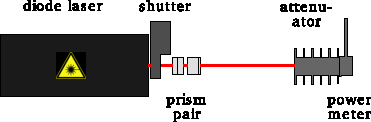
\includegraphics{fig-1}
    \caption{%
        Setup for characterizing the diode laser.
        \parencite[Figure~1]{lab-course/doubling/manual}
    }
    \label{fig:fig-1}
\end{figure}

For measuring the power we just dump the whole beam into a power meter. Since
the power meter become non-linear beyond \SI{20}{\milli\watt} we use an
attenuator in front of it. This will take away a certain fraction of the beam
and allow us to measure higher intensities. The attenuator has to be calibrated
first with small beam powers to allow for a comparison.

% TODO Measure up to 280 mA.
% TODO Measure background.
% TODO Calibrate attenuator.

\subsection{Injection current}

% TODO Plot output versus current.

\subsection{Threshold current}

% TODO Extract threshold.

\subsection{Quantum efficiency}

% TODO Compute differential slope efficiency.
% TODO Compute quantum efficiency from slope.

\subsection{Variable attenuator}
\label{sec:variable_attenuator}

The laser might experience \emph{mode hops} when we adjust the current.
Therefore we do not want to adjust laser power by the current during our
adjustment. We rather want to have an optical way to adjust the beam power. For
this we will use a polarizing beam splitter and a $\lambda/2$-plate in front of
that. By adjusting the polarization of the beam going into the polarizing
splitter we can select the portion of the power advancing to the next parts in
our setup. We extend out setup with a plate and splitter like shown in
Figure~\ref{fig:fig-2}.

\begin{figure}
    \centering
    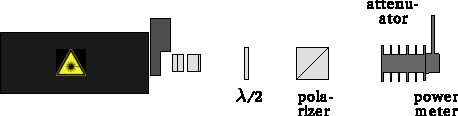
\includegraphics{fig-2}
    \caption{%
        %
        \parencite[Figure~2]{lab-course/doubling/manual}
    }
    \label{fig:fig-2}
\end{figure}

We must obtain a relation of retarder plate angle and output power to use this
later on. There is only one power meter and we want to measure the powers of
both the fundamental and harmonic beam at the same time. We take power
measurements of the fundamental beam in \SI{2.5}{\degree} steps of the retarder
plate.

% TODO Measure power depending on the retarder plate angle.

We expect to see a $\cos^2$ profile, perhaps with a constant offset.

% TODO Fit data.

\subsubsection{Extinction ratio}

% TODO Determine extinction ratio.

\section{Harmonic power}

Now we have the power measurement calibrated. We can determine the power in the
fundamental beam from the angle of the retarder plate. Our setup is extended
with the non-linear crystal and a filter as shown in Figure~\ref{fig:fig-4}.
The blue filter is needed to get rid of the fundamental wave, we only want to
measure the power of the harmonic wave here.

\begin{figure}
    \centering
    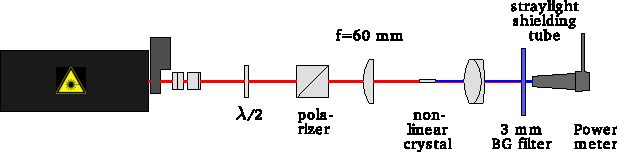
\includegraphics{fig-4}
    \caption{%
        %
        \parencite[Figure~4]{lab-course/doubling/manual}
    }
    \label{fig:fig-4}
\end{figure}

The crystal used here is a $\mathrm{KNbO_3}$ crystal. It has a cross section of
\SI{2}{\milli\meter} times \SI{1.8}{\milli\meter}. It is cut along the b-axis
and has a length of \SI{5}{\milli\meter}. The end faces are coated to avoid
reflections at \SI{987}{\nano\meter} and \SI{494}{\nano\meter}.
\parencite[6]{lab-course/doubling/manual}

% TODO Write about adjustment.

\subsection{Output power optimization}

With the rough optical setup in place we can insert the crystal and optimize
for maximum harmonic power. We slowly heat up the crystal to \SI{36}{\celsius}.
Then we slide it into the focus of our setup.

% TODO Check with paper behind the crystal that one can see something.

The blue harmonic light is focused with an achromatic lens and filtered with an
\SI{3}{\milli\meter} BG40 glass filter. From Figure~3 from
\parencite{lab-course/doubling/manual} we estimate a total transmission
coefficient of \num{0.9} at \SI{494}{\nano\meter}. For the unwanted fundamental
wave we have a transmission coefficient of around $10^{-2.3} = 0.005$.

% TODO Think about the effect of the fundamental wave in our measurement here.

We slightly move and rotate the crystal to optimize the output power.

\subsubsection{Beam waist and Rayleigh length}

% FIXME See whether those numbers actually make sense. Is the correct branch of
% the equations given by Mathematica chosen?

One can let Mathematica solve the
relations describing the beam waist to give an expression for the Rayleigh length
$z_0$:
\[
    z_0 = \piup \frac{n w(z)^2 + \sqrt{n^2 w(z)^4 - 4 \lambda_0^2 z^2}}{2 \lambda_0} \,.
\]
We know that the focal length of the used lens is $f = \SI{60}{\milli\meter}$.
Since the incoming laser beam is collimated, we know that the distance $z$
between the focus and the lens is just this $f$. The diameter of the collimated
beam is given by $w(z) = \SI{3.5 +- 0.5}{\milli\meter}$
\parencite[8]{lab-course/doubling/manual}. Inserting the numbers into the
equation we obtain a Rayleigh length of $z_0 = \SI{<< rayleigh_length_mm
>>}{\milli\meter}$ and a waist of $w_0 = \SI{<< waist_mum >>}{\micro\meter}$.
We obtain a normalized crystal length $\xi = l/b = \num{<< normalized_length
>>}$.

For the optimal case we would need to have $\xi_0 = \num{2.84}$. Given the large
error margin our result $\xi$ could be close enough to $\xi_0$. The more
accurate approach is to perform a one-sample $t$-test. Our null hypothesis is
$\xi = \xi_0$. Can we disprove the null hypothesis, i.e.\ is there no
measurable deviation given the large error of the beam diameter? The test
statistic is $T = \num{<< boyd_kleinman_ttest_t >>}$. Intuitively one can think
of this as the distance of $\xi$ to $\xi_0$ in terms of the standard error
(standard deviation reduced by $\sqrt N$, $N = 1$ is the sample count here).
A look into a table with percentiles of the $t$-distribution tells us that for
a two-sided test with a confidence level of $\alpha = 0.6$ the $|T|$ would have
to be greater than 1.376 for us to reject the null hypothesis
\parencite{wikipedia/student_t}. If we want a higher rejection power, we would
set $\alpha = 0.05$ but would incur a quantile value of 12.71 which $|T|$ would
have to exceed for us to reject the null hypotheses. Therefore we must accept
the null hypothesis and say that the Boyd-Kleinman condition is fulfilled.

The optimal focal length can be derived as follows: We want $l/b = \xi_0 =
2.84$. Therefore we need $z_0 = l/(2\xi_0)$ and
\[
    w_0^2 = \frac{l \lambda_0}{2n\piup\xi_0} \,.
\]
Using the relation for the beam radius we can derive
\[
    z^2 = \sbr{
        \frac{2n \piup w(z)^2 \xi_0}{l \lambda_0} - 1
    } \frac{l^2}{4 \xi_0^2} \,.
\]
Plugging in the numbers we obtain an optimal $f = z$ of \SI{<<
optimal_focal_length_mm >>}{\milli\meter}.

\subsection{Crystal temperature dependence}

Since the index of refraction is temperature depending on our crystal material
we want to measure the temperature dependence. First we cool down to
\SI{27}{\celsius} in steps of \SI{0.5}{\celsius} and then heat up to
\SI{40}{\celsius} in steps of \SI{0.2}{\celsius}.

% TODO Take measurements of power and background at each temperature.

% TODO Plot data such that sinc shape can be seen.
% TODO Try to fit a sinc function.
% TODO Explain why the curve could be asymmetric.

Now that we know the optimal temperature for the crystal, we slowly tune the
temperature to this optimal setting.

\subsection{Input power dependence}

The output power must depend on the input power. As we have calibrated in
Section~\ref{sec:variable_attenuator}, we can choose an input power by rotating
the retarder plate in front of the splitter. We measure the output power while
adjusting the angle of the retarder plate.

% TODO Table with measurements.

% TODO Plot output power versus input power.
% TODO Determine expected relationship.
% TODO Fit model to data.
% TODO Extract frequency doubling efficiency.

\subsection{Input polarization dependence}

By taking out the polarizing beam splitter we can freely adjust the linear
polarization of the light that goes into the crystal. We take a set of
measurements of the output power with different angles of the retarder plate.

% TODO Table with measurements.

% TODO Plot.
% TODO What do we expect for type 1 and type 2?
% TODO Fit the data.
% TODO Are the fit parameters sensible?

\section{Wavelength comparison}

As this experiment is titled \emph{frequency doubling} we except that the
frequency of the incident beam has doubled pretty much exactly. In the
following parts we will compare the two wavelengths with each other and
determine how exact the doubling actually is.

\subsection{Grating}

The first and quick method is using a grating to have a wavelength dependent
diffraction. As the diffraction angle scales with diffraction order $n$ and
wavelength $\lambda$ as a quotient we would expect to see an overlap of the
$n$-th order fundamental wave and the $2n$-th order harmonic wave.

% TODO Increase resolution by using achromatic lens with largest focal length.

% TODO Show all used lengths in a drawing.
% TODO How accurately is the measurement?
% TODO Compare to theoretical resolution.

\subsection{Michelson interferometer}

The rough confirmation of the frequency doubling can be made more precise with
a Michelson interferometer. The setup which we are going to build now is shown
in Figure~\ref{fig:fig-5}.

% TODO Describe how we set this thing up.

\begin{figure}
    \centering
    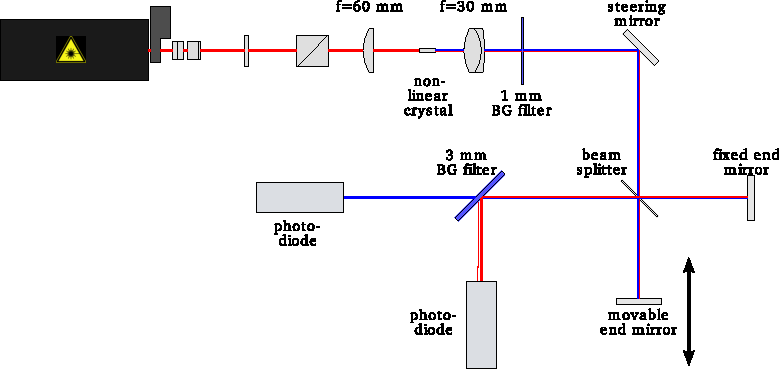
\includegraphics{fig-5}
    \caption{%
        %
        \parencite[Figure~5]{lab-course/doubling/manual}
    }
    \label{fig:fig-5}
\end{figure}

As mentioned in the theory part, the interference intensity $I(\lambda)$
depends on the arm lengths $d_1$ and $d_2$, see
Equation~\eqref{eq:I_of_lambda}. By choosing $d_2$ constant and changing $d_1$,
we have
\[
    \dot I(\lambda) = - \frac12 I_0(\lambda) 
        \sin\del{4 \piup \frac{d_1 - d_2}{\lambda}}
        4 \piup \frac{\dot d_1}{\lambda} \,.
\]
Adding the contributions for $\lambda$ (fundamental) and $\lambda/2$ (harmonic)
together we see that we have
\[
    \dot I_\text{sum}
    =
    - \frac{2 \piup \dot d_1}{\lambda}
    \sbr{
        I_0(\lambda) 
        \sin\del{4 \piup \frac{d_1 - d_2}{\lambda}}
        +
        2 I_0(\lambda/2) 
        \sin\del{8 \piup \frac{d_1 - d_2}{\lambda}}
    } \,.
\]
We expect that the fundamental and harmonic parts in the output of the
interferometer oscillate with different frequencies. Splitting the colors and
displaying this in $x$-$y$-mode on the oscilloscope should give Lissajous
figures with $1:2$ ratio.

Behind the last BG40 filter we have two fast photo diodes. One will receive the
light from the fundamental wave and a negligible part of the harmonic wave. The
other one will receive the harmonic wave and a severely suppressed part of the
fundamental wave. We should be able to take it as a perfect split. Hooking both
photo diodes to the oscillopscope, we obtain some Lissajous figures as shown in
Figure~\ref{fig:lissajous-measured}.

% TODO Take images of the x-y-mode on the oscilloscope.

To get some intuition about the Lissajous figures we have shown a few in
Figure~\ref{fig:lissajous-generated}. The ones that we would expect are in the
first row. If there is some offset we would obtain figures as in the second
row. On the oscilloscope it would actually be figure that seems to be rotating
as the ratio is not exact. With a sufficient exposure time, the figures would
look somewhat like the \enquote{frozen} one generated. In case there is some
other ratio, figures like in the last row would be expected.

\begin{figure}
    \centering
    \begin{subfigure}[c]{0.3\linewidth}
        \centering
        \includegraphics{lissajous_2_0}
        \caption{%
            $r = 2$, $\phi_0 = 0$
            }
        \label{fig:/1}
    \end{subfigure}
    \hfill
    %
    \begin{subfigure}[c]{0.3\linewidth}
        \centering
        \includegraphics{lissajous_2_02}
        \caption{%
            $r = 2$, $\phi_0 = 0.2$
            }
        \label{fig:/1}
    \end{subfigure}
    \hfill
    %
    \begin{subfigure}[c]{0.3\linewidth}
        \centering
        \includegraphics{lissajous_2_1}
        \caption{%
            $r = 2$, $\phi_0 = 1$
            }
        \label{fig:/1}
    \end{subfigure}
    \hfill
    %
    \begin{subfigure}[c]{0.3\linewidth}
        \centering
        \includegraphics{lissajous_21_0}
        \caption{%
            $r = 2.1$, $\phi_0 = 0$
            }
        \label{fig:/1}
    \end{subfigure}
    \hfill
    %
    \begin{subfigure}[c]{0.3\linewidth}
        \centering
        \includegraphics{lissajous_21_07}
        \caption{%
            $r = 2.7$, $\phi_0 = 0.7$
            }
        \label{fig:/1}
    \end{subfigure}
    \hfill
    %
    \begin{subfigure}[c]{0.3\linewidth}
        \centering
        \includegraphics{lissajous_23_24}
        \caption{%
            $r = 2.3$, $\phi_0 = 2.4$
            }
        \label{fig:/1}
    \end{subfigure}
    \hfill
    %
    \begin{subfigure}[c]{0.3\linewidth}
        \centering
        \includegraphics{lissajous_1_0}
        \caption{%
            $r = 1$, $\phi_0 = 0$
            }
        \label{fig:/1}
    \end{subfigure}
    \hfill
    %
    \begin{subfigure}[c]{0.3\linewidth}
        \centering
        \includegraphics{lissajous_1_1}
        \caption{%
            $r = 1$, $\phi_0 = 1$
            }
        \label{fig:/1}
    \end{subfigure}
    \hfill
    %
    \begin{subfigure}[c]{0.3\linewidth}
        \centering
        \includegraphics{lissajous_3_0}
        \caption{%
            $r = 3$, $\phi_0 = 0$
            }
        \label{fig:/1}
    \end{subfigure}
    \hfill
    %
    \caption{%
        Lissajous figures generated with $x(t) = \sin(t)$ and $y(t) = \sin(rt +
        \phi_0)$ and $t \in [0, 8 \piup]$.
        }
    \label{fig:lissajous-generated}
\end{figure}

% TODO Explain the meaning of the oscillograms.
% TODO Determine deviation from 1:2 ratio.
% TODO What causes the deviation?
% TODO Compare with literature values.
% TODO Compute spectral representation of the interferometer.

\end{document}

% vim: spell spelllang=en_us tw=79
